\chapter{PDEs using neural networks} 
\label{chapter3}
\section{Hyperparameters}
Here is the scheme of model tuning followed:
\begin{figure}[h]
    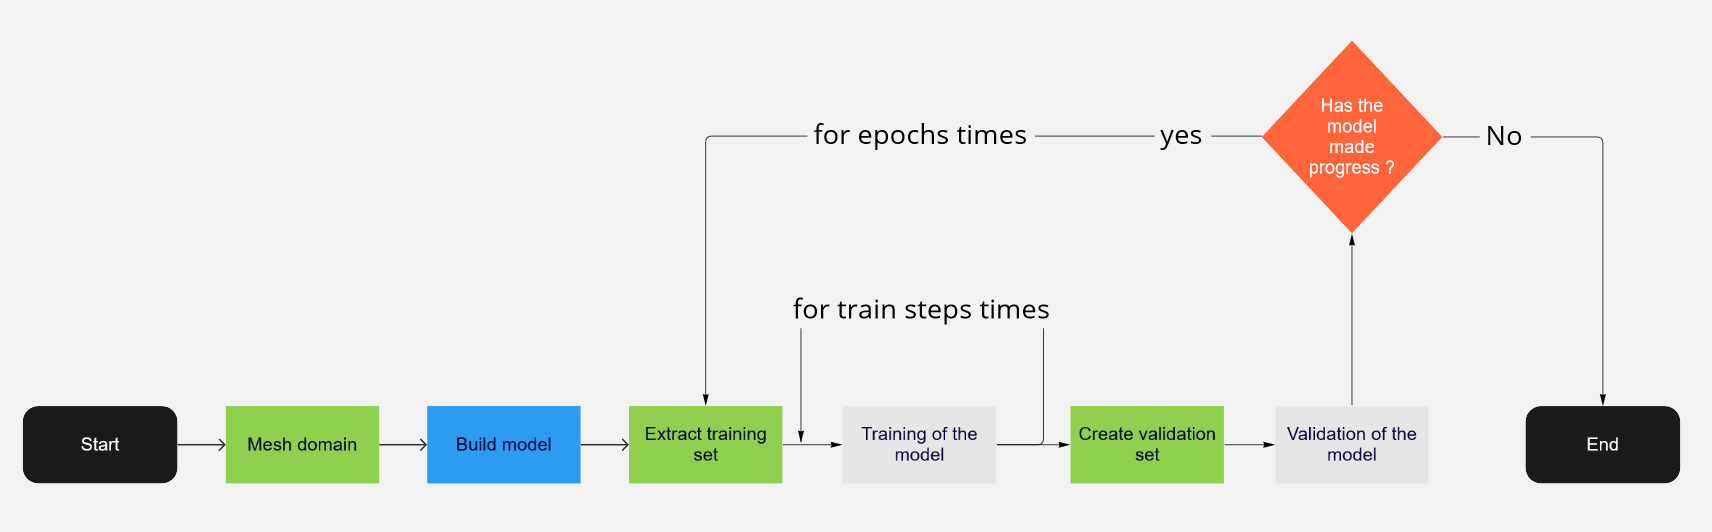
\includegraphics[width=13cm, height=4cm]{images/tuning_model.png}
    \centering
    \caption{scheme of a model tuning}
\end{figure}

The red box involves using an early stopping callback to stop the epoch loop when the model begins to overfit. A \texttt{patience} integer set how far the system will go back in history. If during \texttt{patience} epochs the has not made progress the epoch loop is stopped.
\newline
The hypertuning comes when one wants to construct a model and a training that will end to a low validation error. Let's list all the hyperparameters involved in this scheme applied for the Poisson equation on a square domain:
\begin{itemize}
    \item \texttt{grid\_length}: integer setting the number of points in the domain to \texttt{grid\_length}x\texttt{grid\_length}
    \item \texttt{l\_units}: list of integers depicting the number of hidden layers and the number of neurons per layer of the sequential machine learning model
    \item \texttt{l\_activations}: list depicting the activation functions of each layer of the model
    \item \texttt{noise}: integer in $\{0,1\}$ conditioning the use of a Gaussian layer of mean $0$ after the input layer
    \item \texttt{stddev}: the standard deviation of the Gaussian layer when it is used
    \item \texttt{optimizer}: string depicting the optimizer used
    \item \texttt{learning\_rate}: float setting the learning rate of the previous optimizer
    \item \texttt{epochs\_max}: integer setting the number of maximum epoch loops
    \item \texttt{n\_trains}: integer setting the number of train loops
    \item \texttt{batch\_size}: integer setting the number of points extracted from the mesh to construct the training set at each epoch loop
    \item \texttt{patience}: integer setting how many epoch loops the system can go on without progressing, after that the trial is ended
\end{itemize}

An automatization of the hypertuning by hand and using Keras Tuner has already been led. Nevertheless, some work must still be done to assure a low validation error with minimal cost of time and hardware. A few bugs, impeding a proper convergence, also seems to persist in some of our implementations.

\newpage
\section{Pseudo-code}
\label{pseudo_code}
\begin{algorithm}[H]
    \caption*{Solving PDEs using neural networks (PINN method)}
    \hspace*{\algorithmicindent} \textbf{Input} a,b,c\\
    \hspace*{\algorithmicindent} \textbf{Output} d
    \begin{algorithmic}
    \STATE a $\leftarrow$ c
    \STATE b $\leftarrow$ a
    \STATE \textbf{function} \quad resursion(a,b)
        \bindent
        \RETURN a
        \eindent
    \end{algorithmic}
    \end{algorithm}

\section{Activation functions}
\label{activation}

\newpage
\section{PDE example}
\label{pde_example}
We want to solve the following PDE using the algorithm described on section \ref{pseudo_code} with some activation functions of the section \ref{activation}.
\begin{equation}
    \Delta \psi(x,y) +\psi(x,y)\cdot\frac{\partial \psi(x,y)}{\partial y}= f(x,y) \quad\text{on}\quad \Omega = [0,1]^2  
\end{equation}
with boundary conditions $\psi(0,y)=\psi(1,y)=\psi(x,0)=0$ and $\frac{\partial \psi}{\partial y}(x,1)=2\sin(\pi x)$           
and $f(x, y)=\sin(\pi x)(2-\pi^2y^2+2y^3\sin(\pi x))$. 
\newline
This problem has a analytical solution $\psi_t$ s.t $\psi_t(x, y)=y^2sin(\pi x)$. Thus, to solve it and compare the results we define our loss function like $\mathcal{L} = ||\Delta \psi(x,y) +\psi(x,y)\cdot\frac{\partial \psi(x,y)}{\partial y}-f(x,y) ||_2$  
and the approximated solution like $\psi_a(x,y)=F(x,y)N(x,y)+A(x,y)$ with:
\begin{itemize}
    \item $F(x,y)=\sin(x-1)\sin(y-1)\sin(x)\sin(y)$
    \item $A(x,y)=y\sin(\pi x)$        
\end{itemize}

\section{Jax approach}
\subsection{Jax library}
Jax is a python library built using lax architecture, which makes it high performance and highly recommended for simulations that have a high computational cost. Also, because of the way it is used to implement a neural network, it is possible to parallelize several steps of the simulation so that it runs faster.  
Therefore, due to these characteristics, we chose to do some tests with it.

\subsection{Solving with hyperbolic tangent}
On the image below we can see the results obtained for the PDE of the section \ref{pde_example} using $\tanh$.
\begin{figure}[H]
\begin{subfigure}{0.45\textwidth}
    \centering
    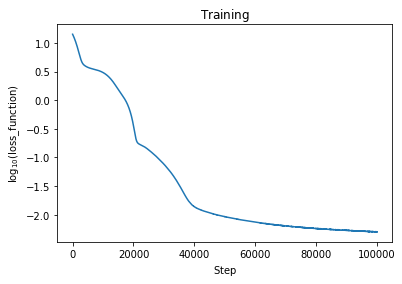
\includegraphics[width=.8\linewidth]{images/NN_Jax_PDE8_files_tanh/NN_Jax_PDE8_18_1.png}
    %\caption{A subfigure}
    \label{fig:sub1}
\end{subfigure}%
\begin{subfigure}{0.45\textwidth}
    \centering
    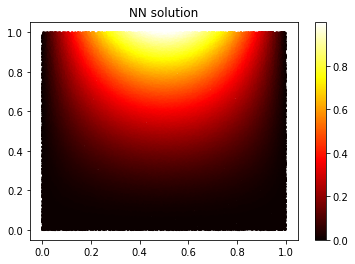
\includegraphics[width=0.8\linewidth]{images/NN_Jax_PDE8_files_tanh/NN_Jax_PDE8_20_0.png}
    %\caption{A subfigure}
    \label{fig:sub2}
\end{subfigure}
\newline
\begin{subfigure}{.45\textwidth}
    \centering
    \includegraphics[width=.8\linewidth]{images/NN_Jax_PDE8_files_tanh/NN_Jax_PDE8_22_0.png}
    %\caption{A subfigure}
    \label{fig:sub3}
    \end{subfigure}
\begin{subfigure}{.45\textwidth}
    \centering
    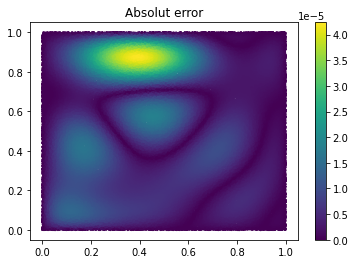
\includegraphics[width=.8\linewidth]{images/NN_Jax_PDE8_files_tanh/NN_Jax_PDE8_24_0.png}
    %\caption{A subfigure}
    \label{fig:sub4}
\end{subfigure}
\caption{Results using Jax and hyperbolic tangent}
\label{fig:test}
\end{figure}

\newpage
\subsection{Solving with sigmoid}
On the image below we can see the results obtained for the PDE of the section \ref{pde_example} using sigmoid.
\vspace{-0.85cm}
\begin{figure}[H]
\begin{subfigure}{.45\textwidth}
    \centering
    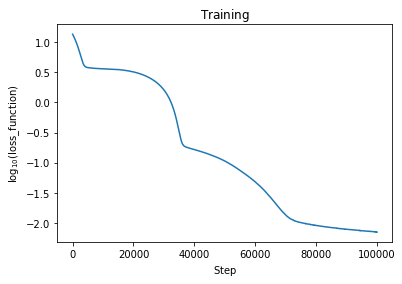
\includegraphics[width=.8\linewidth]{images/NN_Jax_PDE8_files_sigmoid/NN_Jax_PDE8_18_1.png}
    %\caption{A subfigure}
    \label{fig:sub1}
\end{subfigure}%
\begin{subfigure}{0.45\textwidth}
    \centering
    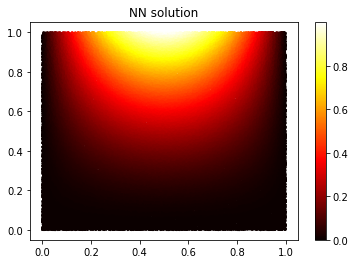
\includegraphics[width=0.8\linewidth]{images/NN_Jax_PDE8_files_sigmoid/NN_Jax_PDE8_20_0.png}
    %\caption{A subfigure}
    \label{fig:sub2}
\end{subfigure}
\newline
\begin{subfigure}{.45\textwidth}
    \centering
    \includegraphics[width=.8\linewidth]{images/NN_Jax_PDE8_files_sigmoid/NN_Jax_PDE8_22_0.png}
    %\caption{A subfigure}
    \label{fig:sub3}
    \end{subfigure}
\begin{subfigure}{.45\textwidth}
    \centering
    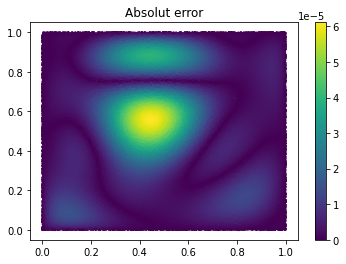
\includegraphics[width=.8\linewidth]{images/NN_Jax_PDE8_files_sigmoid/NN_Jax_PDE8_24_0.png}
    %\caption{A subfigure}
    \label{fig:sub4}
\end{subfigure}
\caption{Results using Jax and sigmoid}
\label{fig:test}
\end{figure}

\vspace{-0.5cm}
\subsection{Solving with gelu}
On the image below we can see the results obtained for the PDE of the section \ref{pde_example} using gelu.
\vspace{-0.45cm}
\begin{figure}[H]
\begin{subfigure}{.45\textwidth}
    \centering
    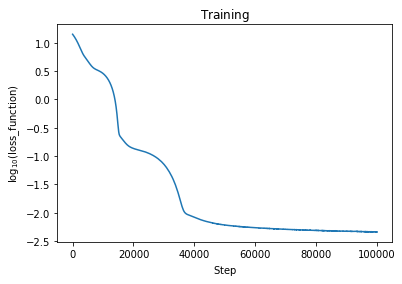
\includegraphics[width=.8\linewidth]{images/NN_Jax_PDE8_files_gelu/NN_Jax_PDE8_18_1.png}
    %\caption{A subfigure}
    \label{fig:sub1}
\end{subfigure}%
\begin{subfigure}{0.45\textwidth}
    \centering
    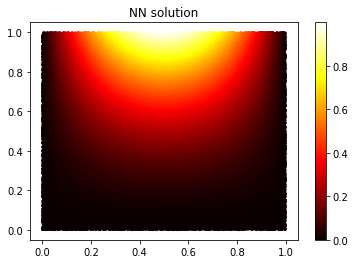
\includegraphics[width=0.8\linewidth]{images/NN_Jax_PDE8_files_gelu/NN_Jax_PDE8_20_0.png}
    %\caption{A subfigure}
    \label{fig:sub2}
\end{subfigure}
\newline
\begin{subfigure}{.45\textwidth}
    \centering
    \includegraphics[width=.8\linewidth]{images/NN_Jax_PDE8_files_gelu/NN_Jax_PDE8_22_0.png}
    %\caption{A subfigure}
    \label{fig:sub3}
    \end{subfigure}
\begin{subfigure}{.45\textwidth}
    \centering
    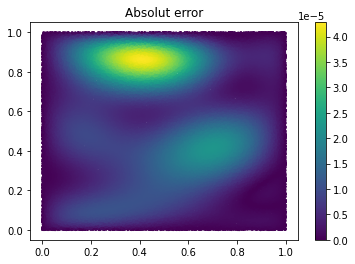
\includegraphics[width=.8\linewidth]{images/NN_Jax_PDE8_files_gelu/NN_Jax_PDE8_24_0.png}
    %\caption{A subfigure}
    \label{fig:sub4}
\end{subfigure}
\caption{Results using Jax and gelu}
\label{fig:test}
\end{figure}

\newpage
\vspace{-0.5cm}
\subsection{Solving with elu}
On the image below we can see the results obtained for the PDE of the section \ref{pde_example} using elu.
\vspace{-0.45cm}
\begin{figure}[H]
\begin{subfigure}{.45\textwidth}
    \centering
    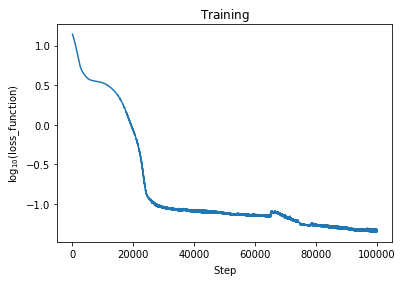
\includegraphics[width=.8\linewidth]{images/NN_Jax_PDE8_files_elu/NN_Jax_PDE8_18_1.png}
    %\caption{A subfigure}
    \label{fig:sub1}
\end{subfigure}%
\begin{subfigure}{0.45\textwidth}
    \centering
    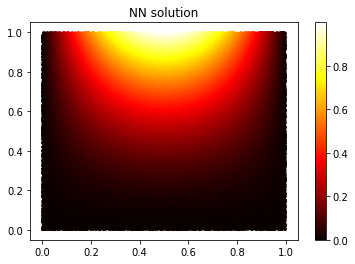
\includegraphics[width=0.8\linewidth]{images/NN_Jax_PDE8_files_elu/NN_Jax_PDE8_20_0.png}
    %\caption{A subfigure}
    \label{fig:sub2}
\end{subfigure}
\newline
\begin{subfigure}{.45\textwidth}
    \centering
    \includegraphics[width=.8\linewidth]{images/NN_Jax_PDE8_files_elu/NN_Jax_PDE8_22_0.png}
    %\caption{A subfigure}
    \label{fig:sub3}
    \end{subfigure}
\begin{subfigure}{.45\textwidth}
    \centering
    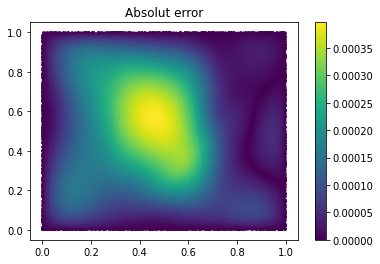
\includegraphics[width=.8\linewidth]{images/NN_Jax_PDE8_files_elu/NN_Jax_PDE8_24_0.png}
    %\caption{A subfigure}
    \label{fig:sub4}
\end{subfigure}
\caption{Results using Jax and elu}
\label{fig:test}
\end{figure}

\vspace{-0.5cm}
\subsection{Solving with relu}
On the image below we can see the results obtained for the PDE of the section \ref{pde_example} using relu.
\vspace{-0.45cm}
\begin{figure}[H]
\begin{subfigure}{.45\textwidth}
    \centering
    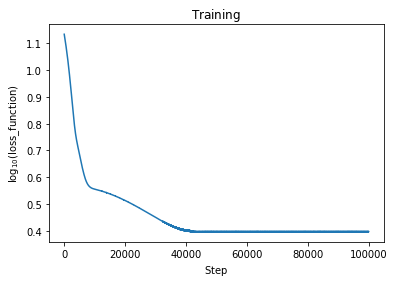
\includegraphics[width=.8\linewidth]{images/NN_Jax_PDE8_files_relu/NN_Jax_PDE8_18_1.png}
    %\caption{A subfigure}
    \label{fig:sub1}
\end{subfigure}%
\begin{subfigure}{0.45\textwidth}
    \centering
    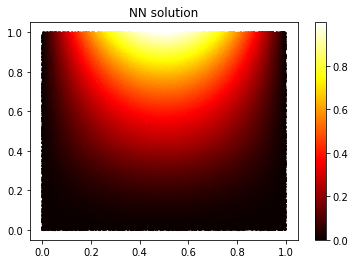
\includegraphics[width=0.8\linewidth]{images/NN_Jax_PDE8_files_relu/NN_Jax_PDE8_20_0.png}
    %\caption{A subfigure}
    \label{fig:sub2}
\end{subfigure}
\newline
\begin{subfigure}{.45\textwidth}
    \centering
    \includegraphics[width=.8\linewidth]{images/NN_Jax_PDE8_files_relu/NN_Jax_PDE8_22_0.png}
    %\caption{A subfigure}
    \label{fig:sub3}
    \end{subfigure}
\begin{subfigure}{.45\textwidth}
    \centering
    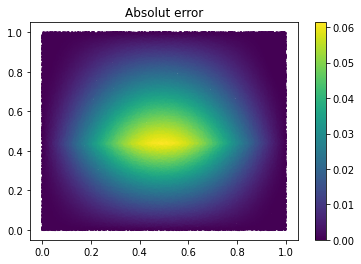
\includegraphics[width=.8\linewidth]{images/NN_Jax_PDE8_files_relu/NN_Jax_PDE8_24_0.png}
    %\caption{A subfigure}
    \label{fig:sub4}
\end{subfigure}
\caption{Results using Jax and relu}
\label{fig:test}
\end{figure}


\vspace{-0.5cm}
\subsection{Analysis}
According to the results obtained, elu and relu activation functions takes longer to converge using the same parameters. Also, it is observed that hyperbolic tangent, gelu and sigmoid provided a smaller absolute error for the same number of iterations.
\newpage

\section{TensorFlow approach}
\subsection{TensorFlow library}
\subsection{Solving with hyperbolic tangent}



\subsection{Solving with sigmoid}

\subsection{Solving with gelu}

\subsection{Solving with elu}

\subsection{Solving with relu}

\subsection{Analysis}


\section{PyTorch approach}
\subsection{PyTorch library}



\subsection{Solving with hyperbolic tangent}



\subsection{Solving with sigmoid}


\subsection{Solving with gelu}

\subsection{Solving with elu}

\subsection{Solving with relu}




\subsection{Analysis}
